\section{Interlinks as sets of superblocks}\label{sec.construction}

In superblock-enabled blockchains, the interlink vector stored in each block $B$
contains one pointer per superblock level $\mu$, namely a pointer to the most
recent superblock preceding $B$ of the respective level $\mu$. This
construction, known as an \emph{interlink list}, is realized by inductively
updating the interlink of the previous block, as shown in
Algorithm~\ref{alg.interlink}. The algorithm works as follows. Trivially,
genesis has an empty interlink vector, which forms our inductive basis. Given a
newly mined block $B'$ which already has an interlink vector (the inductive
hypothesis), we wish to construct the interlink vector to be included in the
next block, which will point to $B'$ itself as well as some of the blocks that
$B'$ points to. This is done by inspecting the existing interlink,
$B'.\textsf{interlink}$, and constructing a new interlink $\textsf{interlink}$
by replacing all the entries in $B'.\textsf{interlink}$ that are of level less
than or equal to that of $B'$ with $B'$ itself.

\import{./}{algorithms/alg.interlink.tex}
\import{./}{algorithms/alg.interlink-set-update.tex}

Here, we make the simple observation that the interlink structure
constructed in this manner often contains \emph{duplicate pointers}. In fact, as
we will show, most of the interlink pointers are duplicate. Space can be saved
by constructing an \emph{interlink set} instead. This construction is shown in
Algorithm~\ref{alg.interlink-set}. The algorithm returns the exact same data
structure as Algorithm~\ref{alg.interlink}, but with duplicates removed. The
algorithm operates as follows. Given an existing interlink set,
$B'.\textsf{interlinkSet}$, it produces a new set $\textsf{interlinkSet}$ which
contains $B'$ and all the same blocks as $B'.\textsf{interlinkSet}$ with the
exception of those that are of equal or inferior superblock level to $B'$.
Naturally, when this interlink set is to be committed to a Merkle tree, it must
be ordered in a canonical matter (for example, by increasing block level) so
that its root can be deterministically reproduced and detected. This canonical
ordering may now not be trivial as was in the case for interlink lists and must
be specified by the implementation.

We remark that it does not matter for security purposes whether duplicates are
removed. The reason is that the prover has access to the whole list of blocks
references within the interlink Merkle tree, and hence can choose the one it
needs. On the other hand, the verifier only needs to ensure that the claimed
superblock level is attained, but this can be done directly by inspecting the
hash sent to it by the prover.

We now analyze the savings attained by the above method. We first analyze the
savings in a thought experiment of an ideal, deterministic execution of the
blockchain protocol. While this setting is not realistic, it provides good
intuition about the interlink structure. Subsequently, we analyze the real
probabilistic blockchain protocol. Consider a blockchain of $n$ blocks.

\begin{definition}[Interlink mask]
Define the \emph{interlink mask} of a block $B$ to be the bitstring containing
one bit per superblock level $\mu$. At the position $\mu$, the bitstring contains
a $1$ if the most recent $\mu$-superblock ancestor of $B$ differs from the most
recent $(\mu+1)$-superblock ancestor of $B$, or if no $(\mu+1)$-superblock
ancestor exists. Otherwise, it contains a $0$.
\end{definition}

This mask contains a $0$ at the position of duplicates which can be eliminated.
To measure the efficiency of our optimization scheme, we wish to count how many
$0$s are contained in the interlink mask of a given block. Consider, for
example, the block highlighted with a dashed border in
Figure~\ref{fig.deterministic}. Its interlink vector will have an interlink mask
of $0101$. The first $0$ is due to the previous block which happened to be a
$1$-superblock. The latter $0$ is due to the most recent $3$-superblock
overshadowing the preceding $2$-superblock.

In our deterministic thought experiment, consider a blockchain which grows as
illustrated in Figure~\ref{fig.deterministic}. In this blockchain, every block
is a $0$-superblock, every other block is a $1$-superblock, every fourth block
is a $2$-superblock and generally every $2^\mu$-th block is a
$\mu$-superblock.
In this thought experiment, the interlink mask behaves like a binary number
which is increased by $1$ after every block is generated. As such, it will be a
$\mu$-digit binary number. As the process passes through all $\mu$-digit binary
numbers, the number of $0$s and $1$s is on average equal. Hence, the savings
obtained in the deterministic case are exactly $50\%$.

\begin{figure*}[h]
\begin{center}
  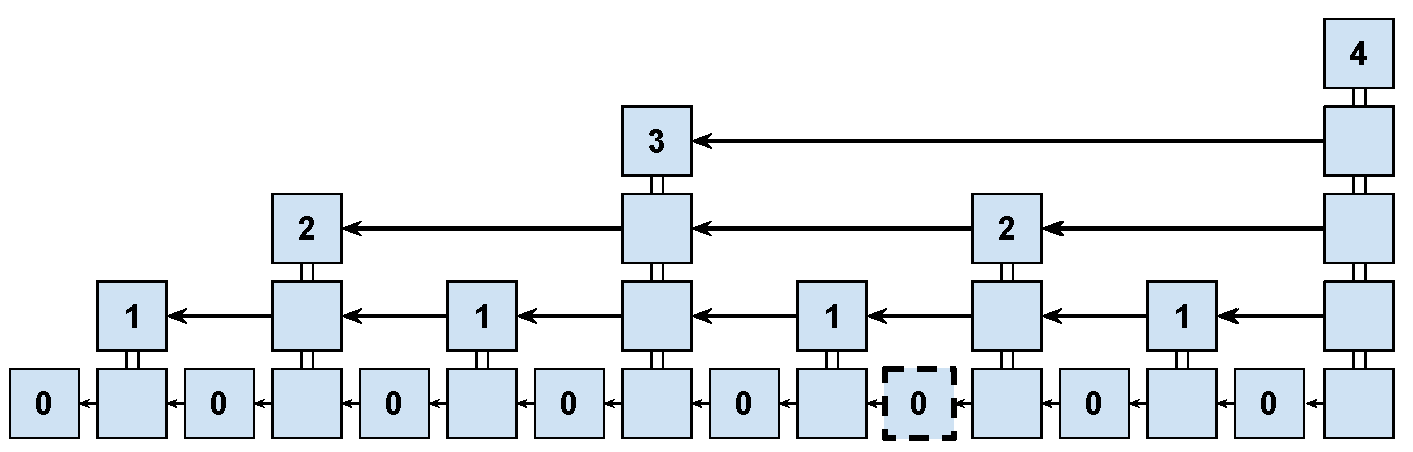
\includegraphics[width=0.95\textwidth]{figures/deterministic-superblocks.pdf}
  \caption{A thought experiment of a deterministically generated blockchain}
  \label{fig.deterministic}
  \end{center}
\end{figure*}

\import{./}{algorithms/alg.tm.tex}

Consider now the probabilistic setting of a real blockchain in an honest execution, where each block
generated has an independent probability of belonging to a given level. The
process of block generation can be modelled precisely as follows. Consider the
Turing Machine illustrated in Algorithm~\ref{alg.tm}. We begin with a one-sided
infinite tape filled with the special symbol $\sqcup$. We then run the machine
illustrated in Algorithm~\ref{alg.tm} repeatedly over the same tape $n$ times.
Once we have completed the $n$ runs, the tape contains a binary string, which
follows the same distribution as the interlink mask of the $n^\text{th}$ block
of a blockchain. Each run of Algorithm~\ref{alg.tm} corresponds to a generation
of a block. The algorithm begins at the position $\mu = 0$ of the tape. It flips
a fair coin $b$. If the coin turns out to be $1$, the machine writes $1$ to the
current position of the tape and exits. This is the event that the block
generated has level exactly $0$. Otherwise, if the coin $b$ is a $0$, then the
block generated has level above $0$, and so the first position of the interlink
mask will be overwritten by a $0$. The machine then advances and
continues to flip coins and overwriting the tape with $0$s until a $1$ coinflip
is attained, at which point it writes a $1$ and halts. The probability of the
machine halting at position $\mu$ or later is $2^{-\mu}$, modeling the
probability of a block being a $\mu$-superblock. The machine overwrites with $0$
the positions in the tape which are of inferior level compared to the block
level it will generate at the given run. This is the same process by which
superblocks of higher level overshadow preceding superblocks of lower levels by
occupying their space with duplicate pointers that can be eliminated.

Let $B^n_\mu \in \{0, 1\}$ denote the random variable containing the value of
the $\mu^{\text{th}}$ digit after $n$ such runs. We have that:

\begin{align*}
\Pr[B^n_\mu = 1] =
\sum_{i = 1}^n 2^{-\mu} \prod_{j = i + 1}^n \sum_{\mu' = 1}^{\mu - 1} 2^{-\mu'} &= \sum_{i = 1}^n 2^{-\mu} \prod_{j = i + 1}^n (1 - 2^{1 - \mu}) &=\\
\sum_{i = 1}^n 2^{-\mu} (1 - 2^{1 -\mu})^{n - (i + 1) + 1} &= \frac{1}{2} (1 - (1 - 2^{1 - \mu})^n)
\end{align*}

Let $B^n$ denote the number of $1$s in the interlink mask after $n$ runs. Its
expectation is then

\[
  \EX[B^n] = \EX[\sum_{\mu = 1}^\infty B^n_\mu] =
  \sum_{\mu = 1}^\infty \frac{1}{2} (1 - (1 - 2^{1 - \mu})^n) =
  \frac{1}{2} \sum_{i = 1}^n (-1)^{i+1} {n \choose i} \frac{2^i}{2^i - 1}
\]

We will now show that the savings from the interlink set technique are significant, specifically that $\EX[B^n] < \frac{1}{2}\lg(n) + O(1)$.

\begin{lemma}
  For any integers $i > 0$ and $k \ge 0$,
  \[
    \frac{2^i}{2^i-1} = \frac{1}{2^{(k+1)i}-2^{ki}} + \sum_{j=0}^k 2^{-ij}
  \]
\end{lemma}
\begin{proof}
  The left-hand side is an infinite geometric series:

  \[
    \sum_{j=0}^\infty (2^{-i})^j = \frac{2^i}{2^i-1}
  \]

  We can split it up at some arbitrary index $k \geq 0$:

  \[
    \sum_{j=0}^\infty (2^{-i})^j = \sum_{j=0}^k 2^{-ij} + \sum_{j=k+1}^\infty (2^{-i})^j
  \]

  Applying the formula for geometric series sum from $j=k+1$ to $\infty$
  on the second term, we obtain:

  \[
    \sum_{j=0}^k 2^{-ij} + \sum_{j=k+1}^\infty (2^{-i})^j
    = \sum_{j=0}^k 2^{-ij} + \frac{2^{-i(k + 1)}}{1  - 2^{-i}}
    = \sum_{j=0}^k 2^{-ij} + \frac{1}{2^{i(k + 1)} - 2^{ik}}
  \]
\end{proof}

\begin{lemma}
  For any positive integers $n$ and $k=\lceil \lg(n) \rceil$,
  \[
    -\sum_{i=1}^n (-1)^i {n \choose i} \sum_{j=0}^k 2^{-ij} < \lg(n) + 2
  \]
\end{lemma}
\begin{proof}
  \begin{align*}
    -\sum_{i=1}^n (-1)^i {n \choose i} \sum_{j=0}^k 2^{-ij}
    &= k+1 - \sum_{j=0}^k \sum_{i=0}^n (-1)^i {n \choose i} 2^{-ij} \\
    &= k+1 - \sum_{j=0}^k \sum_{i=0}^n {n \choose i} (-2^{-j})^i \\
    &= k+1 - \sum_{j=0}^k (1-2^{-j})^n < \lg(n) + 2 \\
  \end{align*}
\end{proof}

\begin{lemma}
  For any positive integer $n$ and $k=\lceil \lg(n) \rceil$,
  \[
    -\sum_{i=1}^n (-1)^i {n \choose i} \frac{1}{2^{(k+1)i} - 2^{ki}} < e
  \]
\end{lemma}
\begin{proof}
  \begin{align*}
    -\sum_{i=1}^n (-1)^i {n \choose i} \frac{1}{2^{(k+1)i} - 2^{ki}}
    &\le \sum_{i=1}^n {n \choose i} \frac{1}{2^{(k+1)i} - 2^{ki}} \\
    &= \sum_{i=1}^n {n \choose i} \frac{1}{2^{ki}(2^i-1)} \\
    &\le \sum_{i=1}^n {n \choose i} \frac{1}{2^{ki}} \\
    &\le \sum_{i=0}^n {n \choose i} \frac{1}{n^i} \\
    &= (1+\frac{1}{n})^n < e \\
  \end{align*}
\end{proof}

\begin{theorem}[Savings]
  $\EX[B^n] < \frac{1}{2}(\lg(n)+2+e)$.
\end{theorem}
\begin{proof}
  \begin{align*}
    \EX[B^n]
    &= -\frac{1}{2} \sum_{i = 1}^n (-1)^i {n \choose i} \frac{2^i}{2^i - 1} \\
    &= \frac{1}{2}((-\sum_{i=1}^n (-1)^i {n \choose i} \sum_{j=0}^k 2^{-ij}) + (-\sum_{i=1}^n (-1)^i {n \choose i} \frac{1}{2^{(k+1)i} - 2^{ki}})) \\
    &< \frac{1}{2}((\lg(n) + 2) + e)
  \end{align*}
\end{proof}

We obtain that $\EX[B^n] < \frac{1}{2}(\lg(n)+2+e)$. Therefore the expected savings are $\lg(n) - \EX[B^n] > \frac{1}{2}(\lg(n)-2-e)$. Solving $\frac{1}{2}(\lg(n)-2-e) > 0$ we obtain that $n > 26$ is sufficient for savings to exist. We conclude that the interlink set method performs better for blockchains with more than $26$ blocks.
